%!TEX TS-program = xelatex
%!TEX encoding = UTF-8 Unicode

\documentclass{scrartcl}

\usepackage[]{geometry}
\usepackage{fontspec}
\usepackage{xcolor}


\setmainfont{DINNextLTPro}[ 
	Path = ../../template/,
	Extension = .otf,
	BoldFont = *-Bold,
	ItalicFont= *-Italic,
	BoldItalicFont= *-BoldItalic,
	UprightFont = *-Regular
	]


\geometry{top =50mm}
\usepackage{enumitem}


\setlist[description]{
	font={\bfseries}
}


\definecolor{footercolor}{HTML}{595959}

\usepackage[]{scrlayer-scrpage}
\clearpairofpagestyles
\chead{
\includegraphics[width=0.6\columnwidth]{../../template/logo.pdf}}
\ofoot{\pagemark}
\cfoot{\small\color{footercolor}
Träger- und Förderverein MINT Oberland | Bruggfeldstraße 5 | 6500 Landeck \par
office@mint.tirol | www.mint.tirol | ZVR-1223647736\par
AT09 3699 0000 0913 4099 | RBRTAT22
}

\usepackage[utf8]{inputenc}
\usepackage{graphicx}

\usepackage[german]{babel}
\usepackage{minutes}
\usepackage{caption}
\usepackage{biblatex}


\newcommand\vereinName{Träger und Förderverein Mint Oberland}
\newcommand\address{Bruggfeldstraße 5, 6500 Landeck}
\newcommand\eMail{office@mint.tirol}
\newcommand\obmann{Philipp Machac}

\minutesstyle{header={list},columns={1},contents={true}}

% ----------------------------------------------------------------

\begin{document}




\begin{Minutes}{Protokoll der Jahreshauptversammlung vom 16.05.2023}

  \subtitle{\vereinName}
  \moderation{\obmann}
  \minutetaker{Simon Abler}
  \participant{
    \nohyphenation {
      Philipp Machac,
      Rainer Haag,
      Simon Abler,
      Michael Netzer,
      Tanja Thurner,
      Eva Machac,
      Marco Handle,
      Reinhold Mungenast,
      Luisa Lercher,
      Eva Hergel,
      Michael Mairhofer
      }
  }

  \minutesdate{16 Mai 2023}
  \starttime{17:00}
  \endtime{18:01}
  \location{Lantech Seminarraum}
  %\missing{}
  \maketitle
  \newpage

  % Header end ---------------------------------------------------------
  \topic{Begrüßung durch den Vorsitzenden des Vorstands}
  Begrüßung durch Obmann \obmann.
  \subtopic{Feststellung der Beschlussfähigkeit}
  Beschlussfähigkeit wurde festgestellt.
  \subtopic{Verlesung des Sitzungsprotokolls vom 24.10.2022}
  Antrag auf Nichtverlesen des letzten Sitzungsprotokolls wurde von Marco Handle eingebracht. Dies wurde einstimmig angenommen. 


  %---------------------------------------------------------

  \topic{Ansprache des Obmannes}
  \obmann  dankt den Unterstützern und Sponsoren, speziell auch den anwesenden Vertreter der Industriellenvereinigung.
  Es folgt eine kurze Zusammenfassung und Vorstellung des Vereins MINT:
  \begin{itemize}
    \item Ziele: Kinder und Jugendliche fördern
    \item Abwanderung verhindern
    \item Unsere Region stärken
  \end{itemize}
  Geplante Maßnahmen:
  \begin{description}
    \item [Elementarpädagogik:] Im Bereich der Elementarpädagogik wird aktiv versucht, die Konzepte, die im Zuge der Mint Strategie von der Industriellenvereinigung ausgearbeitet wurden, in unser Programm einzubauen.
    \item [Volksschule:] wird schon interessanter für unsere Ziele, Vorträge und Exkursionen Interesse wecken
    \item [SEK1:] Realistisches Berufsbild vermitteln, zB. über Workshops im MINT Lab, MINT durch Vorträge neutraler Partner an der Schule präsentieren
    \item [SEK2:] Region sollte besser präsentiert werden, Stichwort: \glqq Auch bei uns gibt es attraktive Arbeitsgeber\grqq{}
    \item [Bevölkerung:] Bewusstseinsschaffung in der Bevölkerung
  \end{description}

  %---------------------------------------------------------

  \topic{Projektvorstellungen}

  \subtopic{MINT-Woche und 2022}
  Vorstellung des Projektes durch \obmann.\\

  Das Konzept der berufspraktischen Wochen sieht vor, dass die Kinder eine Woche lang ein Unternehmen besuchen. 
  Jedoch hat sich gezeigt, dass es für die Unternehmen schwierig ist, dies umzusetzen. 
  Daher möchten wir den Jugendlichen einen Ausblick über mehrere Firmen innerhalb einer Woche bieten. 
  Auf diese Weise können die Schülerinnen und Schüler in einer Woche mehrere Unternehmen kennenlernen, anstatt nur ein Unternehmen zu besuchen. \\
  In den vergangenen Mint Wochen wurden Themen wie Automatisierung, Elektrotechnik, Netzwerktechnik, Programmieren und auch handwerkliche 
  Tätigkeiten wie das Spleißen von LWL-Kabeln und die Arbeit als Elektroinstallateur behandelt. 
  Dadurch haben wir ein abwechslungsreiches Programm geschaffen. 
  Derzeit finden die Veranstaltungen zentral im Lantech statt, wo auch der Transport zu externen Firmen organisiert wird. \\
  Es ist wichtig zu betonen, dass die Mint Woche flexibel auf die Bedürfnisse aller Schulen abgestimmt ist. \\
  Wir werden weitere Maßnahmen ergreifen, um für dieses Modell mehr Werbung zu machen und es auch auf den Bezirk IMST auszuweiten. 
  Die Kinder nehmen das Modell positiv an, und es ist interessant festzustellen, dass jeder Schüler einen anderen Bereich als Favoriten wählt.
  
  \subtopic{MINT-Lab Oberland}
  Präsentation und Vorstellung durch \obmann.\\

  Anknüpfend an das Fablab wurde das Modell auf Schulen und Workshops übertragen. Das Ziel, für interessierte Personen aus der Umgebung offen zu sein, wird weiterhin angestrebt. Es handelt sich um ein Förderprojekt in Zusammenarbeit mit RegioL, bei dem 105.000€ investiert wurden. Davon wurden 60\% (71.727€) gefördert, während der Verein den Restbetrag aufbrachte. In Kooperation mit dem Gymnasium Landeck konnten wir geeignete Räumlichkeiten finden, da das Gymnasium großes Interesse zeigte. Der Standort in Landeck ist ideal, da er mit öffentlichen Verkehrsmitteln gut erreichbar ist (Bahnhof und Bus in der Nähe). Zudem wurden uns die Räumlichkeiten kostenlos zur Verfügung gestellt.

  Die Aufgabenverteilung sieht vor, dass der Verein die Ausstattung bereitstellt, während die Bildungseinrichtung das Lehrpersonal zur Verfügung stellt. Die Workshops finden jeden Mittwoch statt und decken drei Bereiche des Mintlabs ab: Mintlab Technik mit Themen wie Beebot, Programmierung und Löten; Mintlab Kreativ, da Programmierer auch Kreativität benötigen. Hier können auch fächerübergreifende Projekte wie Sticken, Nähen und Schneiden mit dem Lasercutter durchgeführt werden. Zudem gibt es das Biochem Lab mit verschiedenen Workshops zu den Themen Chemie und Biologie.
  
  Bei der Anmeldung müssen die Teilnehmer drei Workshops aus den drei Lab-Bereichen auswählen. Hier einige Zahlen zum Mintlab: Es wurden 14 Volksschulen erreicht, es fanden 105 Workshops statt, an denen 700 Schüler teilnahmen. Insgesamt wurden 6.300 Minuten an Workshops durchgeführt. Zusätzlich gab es 12 Besuche in Schulen und 2 Fortbildungen für Lehrer. Die Freischaltung der Workshops erfolgte im Oktober 2022, und innerhalb von drei Wochen waren die meisten Plätze für das Schuljahr ausgebucht. Dies hat uns gezeigt, dass ein Vormittag zu wenig ist (Abstimmung mit der Bildungsdirektion erforderlich) und dass diese Workshops auch in die Schulen gebracht werden können, um das Konzept des Labs breiter zu streuen. Allerdings sollten Workshops, die größere Geräte erfordern, wieder im Lab stattfinden. Hauptsächlich werden die Workshops von Lehrern des Gymnasiums geleitet, es ist jedoch auch ein Lehrer einer Neuen Mittelschule aus Zams beteiligt. Die Planungen für den Herbst laufen bereits, und in diesem Jahr wurden bereits einige Anschaffungen getätigt.
  
  \subtopic{Coding4Kids Herbstkurs}
  Um das Thema Mint in die Freizeit zu integrieren, können wir Technikbegeisterten (\glqq MINI Nerds\grqq{}) eine Kooperation mit der Initiative Coding4Kids anbieten. Wir können ein Semesterprogramm entwickeln, das Ferienveranstaltungen umfasst. Mint Oberland hat bereits zwei Trainer/-innen organisiert, um eine Veranstaltung mit 8 Teilnehmern durchzuführen. Die Termine wurden zur Hälfte im Mintlab und zur Hälfte online abgehalten. Das Feedback der Kinder zeigte, dass sie es bevorzugen, alle Termine in Präsenz abzuhalten. Daher werden wir versuchen, die Veranstaltung aufrechtzuerhalten und eine neue Reihe von Terminen zu organisieren. Ein Tag der Veranstaltung fand auch lokal bei Firmen im Lantech statt.
  %---------------------------------------------------------

  \topic{Beschlussfassung über eingelangte Anträge}
  Keine Anträge eingelangt.

  \topic{Entgegennahme und Genehmigung des Rechenschaftsberichts und des Rechnungsabschlusses unter Einbindung der Rechnungsprüfer}
  Bericht von Rainer Haag:\\\\
  \textbf{Vorstellung Finanzbericht 2021 / 2022}

  \begin{figure}[h!]
    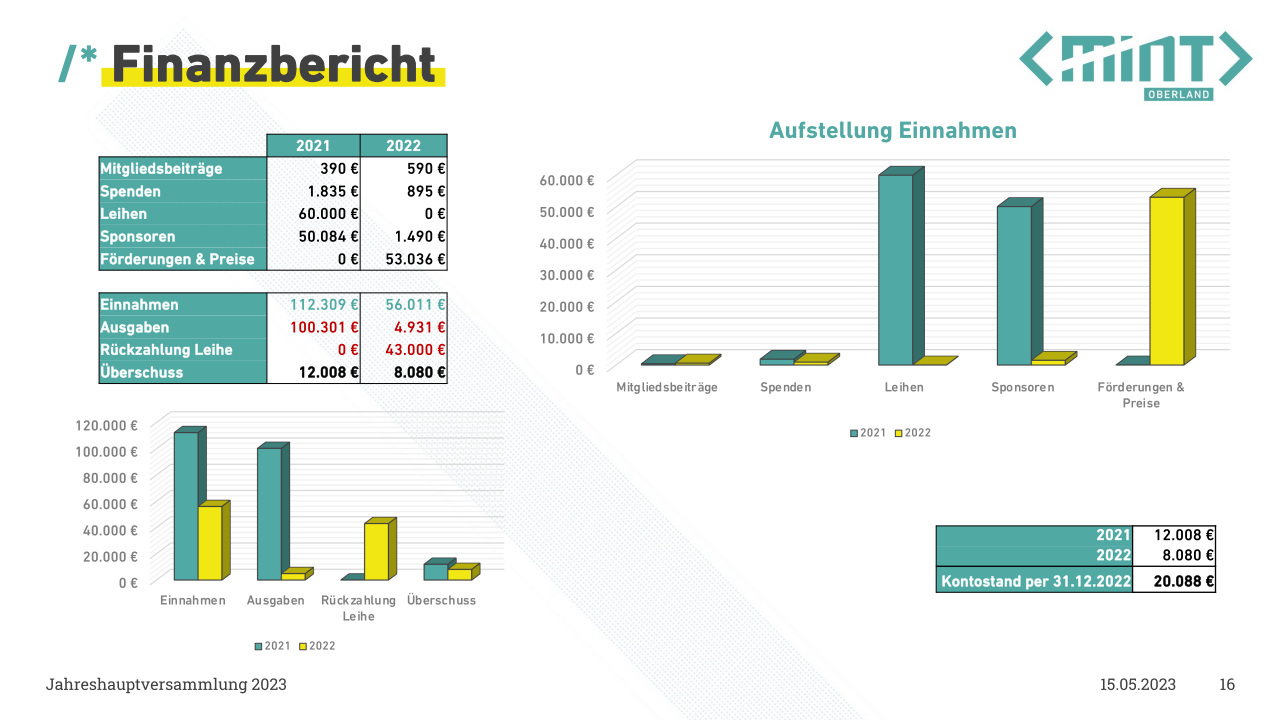
\includegraphics[width=\linewidth]{finanzbericht.png}
    \caption{Finanzbericht 2021 / 2022}
    \label{fig:Finanzbericht}
  \end{figure}

  Kassenbericht, mit Stichtag 31.12.2022. Siehe Abbildung \ref{fig:Finanzbericht}.\\\\
  \textbf{Prognose 2023}

  Die Mitgliederzahl steigt kontinuierlich, und nun sollen auch die Folder eingesetzt werden, um neue Mitglieder zu werben. Zusätzlich hat der Betreuer für Biochemie einen Experimentierkoffer entwickelt, der Tirolweit verkauft wird. Der Verein unterstützt die Schulen durch Förderungen beim Erwerb dieser Koffer. In diesem Jahr wurde auch eine Stickmaschine angeschafft, nachdem das Lehrpersonal an uns herangetreten ist und Schwierigkeiten hatte, die Mädchen abzuholen. Die programmierbare Stickmaschine bietet hier eine Lösung. Des Weiteren wurden Beebots für mehrere Gruppen angeschafft, zusätzlich zu den bereits vorhandenen 3D-Druckern wurden auch 3D-Stifte angeschafft.
  
  Wir arbeiten an neuen Projekten in Zusammenarbeit mit der Jungen Uni und dem Verein Klasse Forschung. Ein Projekt befasst sich mit Bildung und Produktionstechnik und wird durch eine Förderung der FFG unterstützt.  \\\\
  \textbf{Weitere Projekte}

  Evaluation für Minilabs:
  Im Rahmen der Evaluierung für Minilabs suchen wir noch nach großzügigen Sponsoren. Das Ziel ist die Anschaffung von erschwinglichen, kleineren Labs an Schulen. Ein Beispiel dafür ist das Minilab in Kappl, das auch von der Volksschule Ischgl genutzt werden kann.

  Des Weiteren arbeiten wir eng mit der Mintkoordinationsstelle Tirol zusammen, um Elementarpädagogik-Kits wie die Spürnasenecke und Forscherräume einzuführen. In Landeck wird derzeit ein neuer Kindergarten gebaut, und wir haben uns aktiv dafür eingesetzt und unsere Bedürfnisse angemeldet.
  
  Es sind bereits viele Unternehmen auf uns zugekommen und möchten uns unterstützen. Wir werden jedoch erst bei einem konkreten Projekt auf diese Unternehmen zugehen und ihre Unterstützung einfordern.\\\\
  \textbf{Bericht der Kassenprüfer}

  Kassaprüfer Reinhold Mungenast: \glqq Die Kasse wurde am vergangenen Freitag geprüft und es wurden keine Beanstandungen festgestellt. Die Kasse wurde ordnungsgemäß geführt.\grqq{}

  \subtopic{Entlastung des Vorstands}
  \Onevote{Entlastung des Vorstandes. Abgestimmt durch Handzeichen, 17:41 }{8}{0}{0}

  %---------------------------------------------------------

  \topic{Neuwahlen}
  Laut den Statuten sind alle 2 Jahre Neuwahlen vorgesehen. Bisher bestand der Vorstand aus drei Mitgliedern, jedoch stehen uns große Mammutprojekte bevor. Aus diesem Grund haben wir beschlossen, das Team zu erweitern und weitere Mitglieder in den Vorstand aufzunehmen.
  Der Vereinsvorstand hat einen Wahlvorschlag erstellt:
  
  \begin{description}
    \item[Obmann:] Philipp Machac, 6500 Landeck
    \item[Obmann-Stv.:] Luisa Lercher, 6511 Zams
    \item[Schriftführer:] Simon Abler, 6500 Landeck
    \item[Schriftführer-Stv.:] Eva Hergel, 6500 Landeck
    \item[Kassier:] Rainer Haag, 6511 Zams
    \item[Kassier-Stv.:] Marco Handle, 6500 Landeck
  \end{description}


  \noindent  Die Neuwahl wurde von Tanja Thurner durchgeführt. Die Namen der Kandidaten wurden laut vorgelesen.\\
 \Onevote{Neuwahl des Vorstandes. Abstimmung des Wahlvorschlages durch Handzeichen, 17:49 }{5}{0}{0}\leavevmode\newline
 
 \noindent Alle Kandidatinnen / Kandidaten haben die Wahl angenommen.
  Der Obmann dankt allen Anwesenden und begrüßt herzlich den neuen Vorstand.\\

  \topic{Allfälliges}
  Machac bedankte sich für die Unterstützung und betonte, dass das Team breiter aufgestellt werden solle, da große Mammutprojekte anstünden.

  Machael Netzer von der Industriellenvereinigung erwähnte, dass die Mint Koordinierungsstelle in Tirol den Verein unterstützen. Er betonte, dass Mint Oberland als Vorzeigeprojekt gilt und empfahl, dass sich Mint Oberland am Mint Region Güte Siegel beteiligen sollte. Es wurde vorgeschlagen, dass Mint Oberland das Siegel wahrnehmen sollte.
  Machac informierte darauf, dass es einen weiteren Termin mit Daniela Lehmann geben wird und dass möglicherweise auch die Schulen in die Gespräche einbezogen werden können.
  Haag erklärte, dass es zwar kein Sponsorengeld für das Siegel gebe, jedoch sei es wichtig, dass sowohl der Verein als auch die Schulen das Siegel wahrnehmen sollten. Es wäre eine erfreuliche Entwicklung, wenn Mint Oberland die ersten wären, die das Siegel erhalten.
  
  Netzer erkundigte sich, ob das Minilab dasselbe wie die Spürnasenecke sei.
  Haag antwortete, dass dies im Prinzip zutreffe. Es würden den Schulen kleine Geräte zur Verfügung gestellt, die in einem Raum Platz finden. Zudem fügte er hinzu, dass der Verein durch die Obmann-Stellvertreterin nun auch mehr Expertise im Bereich der Elementarpädagogik hätten.
  Die Industriellenvereinigung erwähnte, dass sie Möglichkeiten sehe, einige Minilabs im nächsten Jahr ins Sponsoring aufzunehmen.
  Machac gab bekannt, dass vor der Verteilung der finanziellen Mittel zunächst eine Erhebung durchgeführt werden solle, um festzustellen, welche Ressourcen bereits an den Schulen vorhanden seien. Dadurch könnten die finanziellen Mittel gezielt eingesetzt werden.

  \vspace{0.2\textheight}

  \signature{Obmann, \obmann}
  \hspace{0.2\columnwidth}
  \signature{Schriftführer, Simon Abler}
\end{Minutes}

% ----------------------------------------------------------------

\end{document}
% ----------------------------------------------------------------
